\section{The Dashboard}

The last thing we wanted to implement for the project was a small dashboard were students would have been able to track the lessons they attended for each course, together with some overview statistics. Originally, we would have liked to implement it by integrating it with iCorsi on the Moodle platform. Unfortunately, after consulting the eLab we concluded that it was not possible, due to several problems:

\begin{itemize}
	\item Moodle adopts its own plugin systems for additions to the platform; the modules use their own paradigm, and require knowledge of PHP (which we never tried);
	\item Even if we wanted to try to write a Moodle plugin in PHP, the eLab wouldn't allow us to develop the plugin directly on the iCorsi platform; they could have set up a test instance of Moodle for us, but it would have taken some time; 	\item They would have to give us a test instance of the databases used for storing the student's informations, and we would have to understand its structure and complement it with new tables/fields required to store our own informations.
\end{itemize}

These issues made the Moodle integration not viable, so we had to settle with our own backend (discussed in the previous chapter) and provide the dashboard as a separate application.

\paragraph{}
To implement it, we chose to adopt state of the art web technologies: the application is implemented using \textbf{AngularJS}, and we secured it by implementing the protocol for \textbf{JSW} (Javascript Web Token) authentication.

\paragraph{}
When the application is started, it will require the student to log in using his/her iCorsi credentials:

\begin{center}
	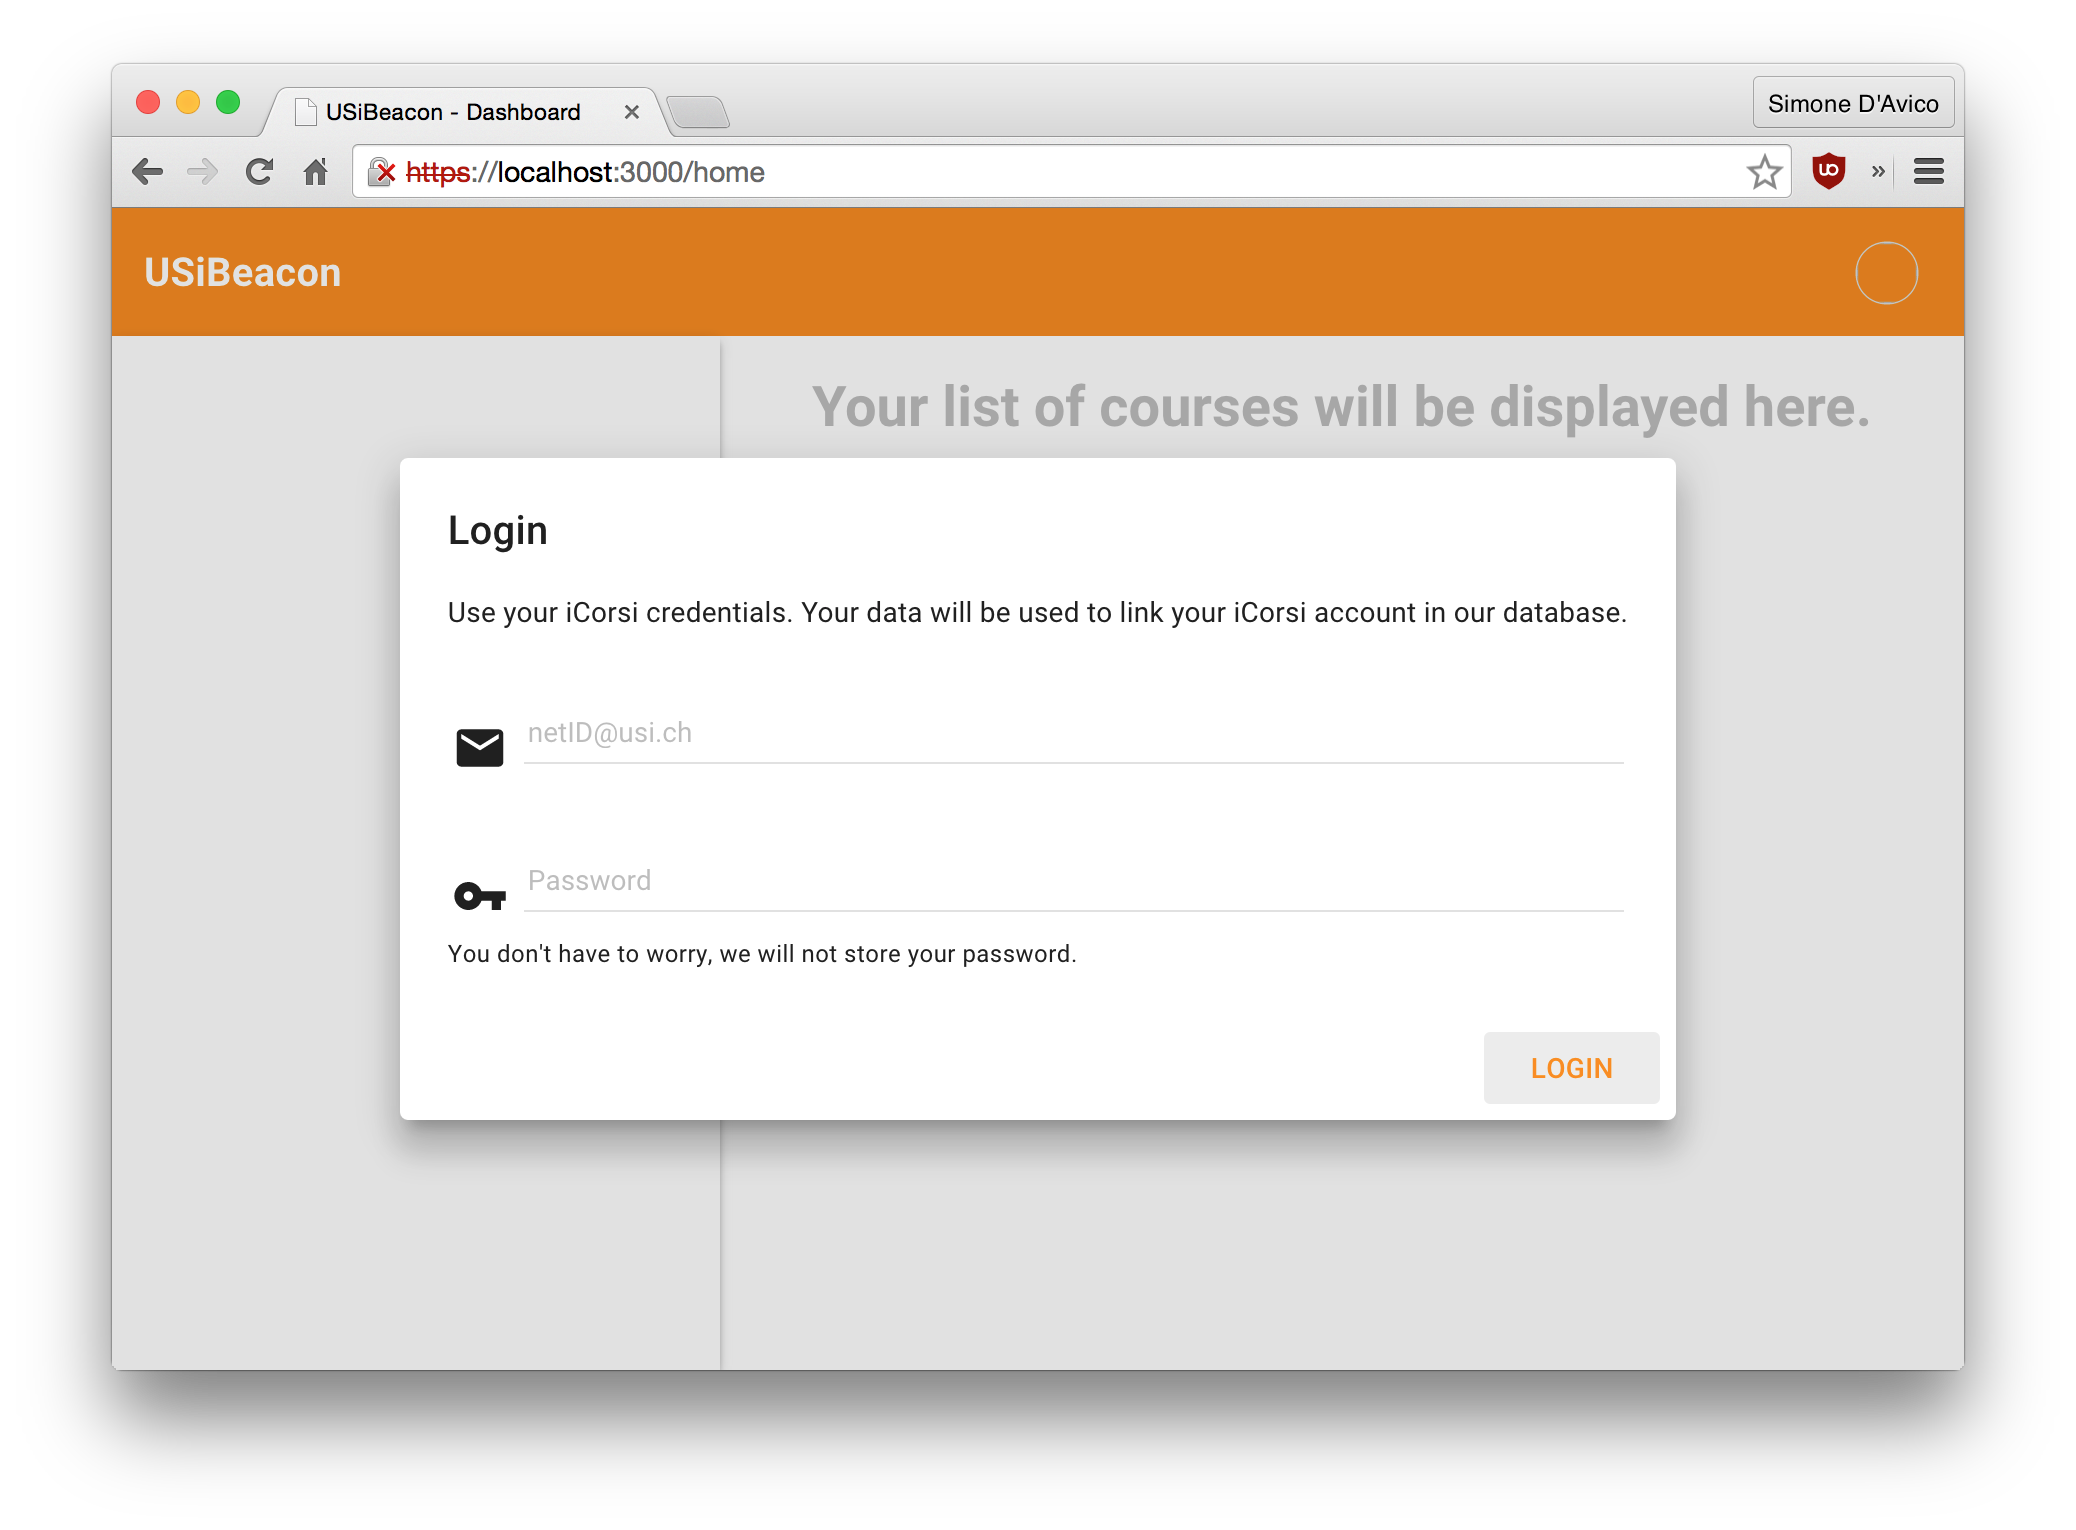
\includegraphics[scale=0.4]{img/dashboard-login}
\end{center}

On login, the application will store the JWT token received by the backend, which will be valid for 7 days from its creation. After the expiration, the student will have to login again. This is what the student will see:

\begin{center}
	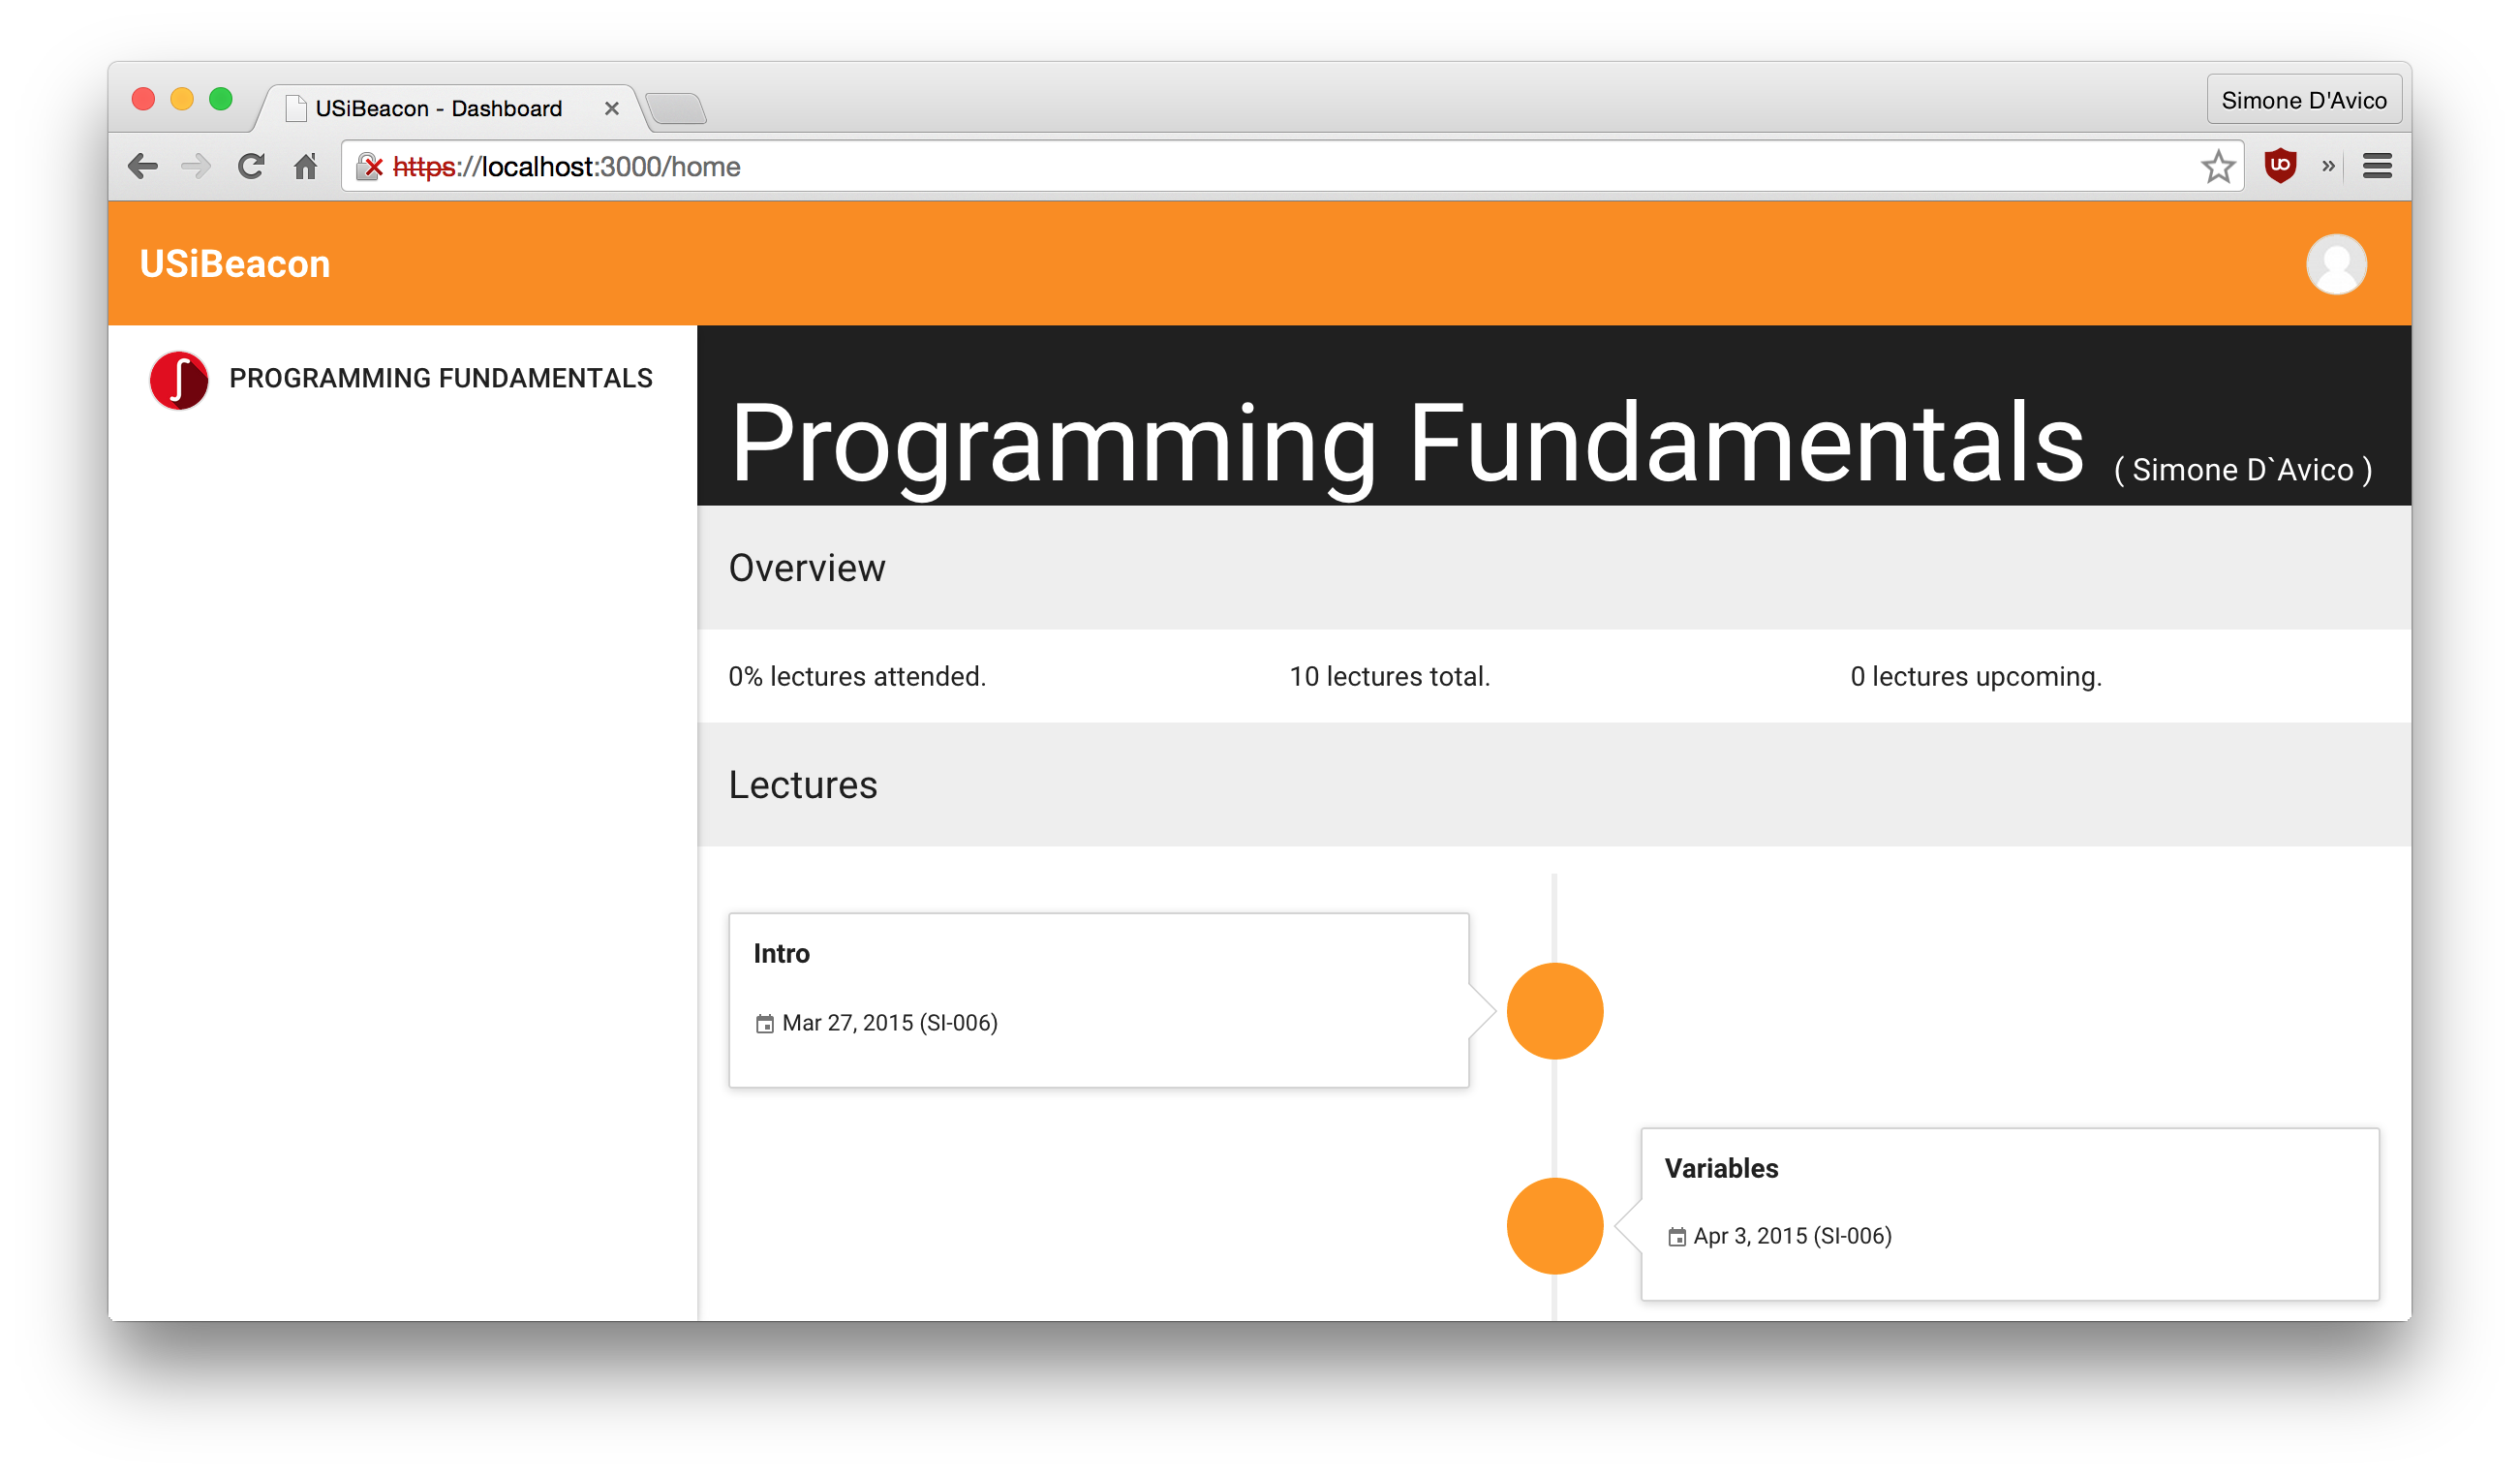
\includegraphics[scale=0.3]{img/dashboard-timeline}
\end{center}

In the overview for each lecture, the student will be able to see the percentage of lessons attended for a given course, the total number of lectures, and the number of upcoming lectures. He/she will also be able to look at a timeline of all the lectures of the course, where each lessons he/she attended will be ticked.